%%%%%%%%%%%%%%%%%%%%%%%%%%%%%%%%%%%%%%%%%
% a0poster Landscape Poster
% LaTeX Template
% Version 1.0 (22/06/13)
%
% The a0poster class was created by:
% Gerlinde Kettl and Matthias Weiser (tex@kettl.de)
% 
% This template has been downloaded from:
% http://www.LaTeXTemplates.com
%
% License:
% CC BY-NC-SA 3.0 (http://creativecommons.org/licenses/by-nc-sa/3.0/)
%
%%%%%%%%%%%%%%%%%%%%%%%%%%%%%%%%%%%%%%%%%

%----------------------------------------------------------------------------------------
%	PACKAGES AND OTHER DOCUMENT CONFIGURATIONS
%----------------------------------------------------------------------------------------

\documentclass[a0,landscape]{a0poster}

\usepackage{multicol} % This is so we can have multiple columns of text side-by-side
\columnsep=100pt % This is the amount of white space between the columns in the poster
\columnseprule=7pt % This is the thickness of the black line between the columns in the poster

\usepackage[svgnames]{xcolor} % Specify colors by their 'svgnames', for a full list of all colors available see here: http://www.latextemplates.com/svgnames-colors

\usepackage{times} % Use the times font
%\usepackage{palatino} % Uncomment to use the Palatino font

\usepackage{graphicx} % Required for including images
\graphicspath{{figures/}} % Location of the graphics files
\usepackage{booktabs} % Top and bottom rules for table
\usepackage[font=large,labelfont=bf]{caption} % Required for specifying captions to tables and figures
\usepackage{amsfonts, amsmath, amsthm, amssymb} % For math fonts, symbols and environments
\usepackage{wrapfig} % Allows wrapping text around tables and figures
\usepackage{comment}
\usepackage{bm}
\usepackage{anyfontsize}
\usepackage{multirow}

\usepackage{sidecap}

\newcommand{\bmu}{\boldsymbol{\mu}}
\newcommand{\bK}{\boldsymbol{\mathrm{K}}}
\newcommand{\bM}{\boldsymbol{\mathrm{M}}}
\newcommand{\mbf}[1]{{\boldsymbol{\mathbf{#1}}}}
\renewcommand{\bm}{\mbf}

\usepackage{subfigure}

\usepackage{parskip}

\usepackage{url}

\usepackage{float} 


\begin{document}

%----------------------------------------------------------------------------------------
%	POSTER HEADER 
%----------------------------------------------------------------------------------------

% The header is divided into three boxes:
% The first is 55% wide and houses the title, subtitle, names and university/organization
% The second is 25% wide and houses contact information
% The third is 19% wide and houses a logo for your university/organization or a photo of you
% The widths of these boxes can be easily edited to accommodate your content as you see fit

\begin{centering}{\fontsize{100}{120} \selectfont \color{NavyBlue} \textbf{Metropolis-Hastings GAN} \color{Black}}\\ % Title
%\Huge\textit{Can Bayes help mode collapse?}\\[1cm] % Subtitle
\Huge \textbf{Ryan Turner, Jane Hung, Jason Yosinski, Yunus Saatci}\\ % Author(s)
\huge Uber AI Labs \\ % University/organization
\end{centering}
%

%


\begin{comment}
\begin{minipage}[b]{0.04959\linewidth}
\includegraphics[width=20cm]{logo.png} % Logo or a photo of you, adjust its dimensions here
\end{minipage}
\end{comment}

\vspace{1cm} % A bit of extra whitespace between the header and poster content

%----------------------------------------------------------------------------------------

\begin{multicols}{3} % This is how many columns your poster will be broken into, a poster with many figures may benefit from less columns whereas a text-heavy poster benefits from more

%----------------------------------------------------------------------------------------
%	ABSTRACT
%----------------------------------------------------------------------------------------

%\color{Navy} % Navy color for the abstract


%----------------------------------------------------------------------------------------
%	INTRODUCTION
%----------------------------------------------------------------------------------------

\Large

\section*{\fontsize{67.1}{82} \selectfont \color{NavyBlue} Generative Adversarial Networks \color{Black}}
\setlength\labelsep   {\dimexpr\labelsep + 0.5em\relax}  
\setlength\leftmargini{\dimexpr\leftmargini + 0.5em\relax}
\vspace{-.5in}
\begin{itemize}
\item Have two neural networks, $G$ and $D$, competing against each other. 
\item $G$ attempts to fool $D$ by generating datapoints which are, from $D$'s perspective, indistinguishable from real datapoints.
\item $D$ in turn simply tries to classify samples coming from $G$ as fake and actual datapoints as real.
\item If this adversarial game converges, it can generate amazingly realistic samples.
\end{itemize}
\textbf{Learning Objective:}
\textcolor{MidnightBlue}{
  \begin{align}
    \underset{G}{\text{min }}\underset{D} {\text{max }} V(D,G) = \mathbb{E}_{\bm{x} \sim p_{\text{data}}(\bm{x})} [\log D(\bm{x})]
    + \mathbb{E}_{\bm{z} \sim p(\bm{z})} [\log(1-D(G(\bm{z})))] \nonumber
  \end{align}}
%\begin{figure}[H]
\begin{centering}
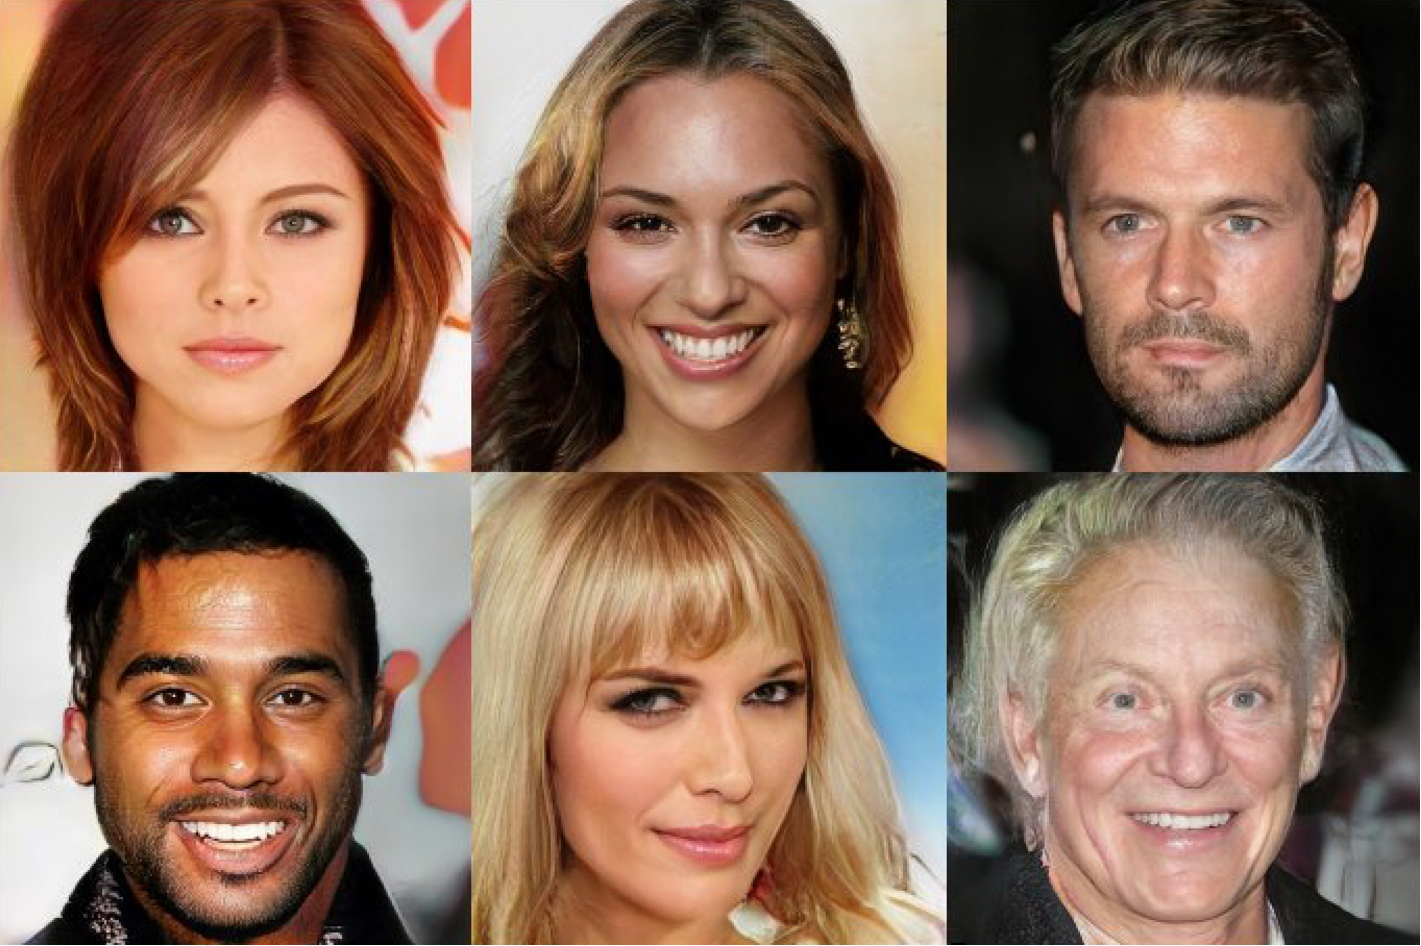
\includegraphics[width=.1\textwidth]{goodsamples.pdf} \\
\small High resolution samples generated by \emph{Karras et. al, arXiv 1710.10196} \\
\end{centering}
%\caption{High resolution samples generated by \emph{Karras et. al, arXiv 1710.10196}}
%\end{figure}
\vspace{-.8in}

\section*{\fontsize{67.1}{82} \selectfont \color{NavyBlue} MH GANs \color{Black}}
TODO
\begin{figure}[H]
\centering
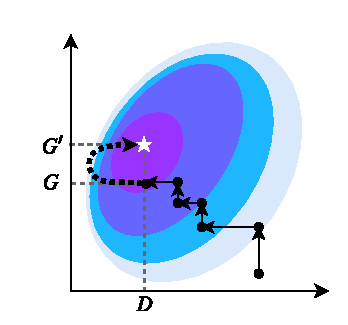
\includegraphics[width=.25\textwidth]{../figures/coord_descent.pdf}
\end{figure}

\section*{\fontsize{67.1}{82} \selectfont \color{NavyBlue} Results on a Synthetic Dataset \color{Black}}
\begin{figure}[H]
\centering
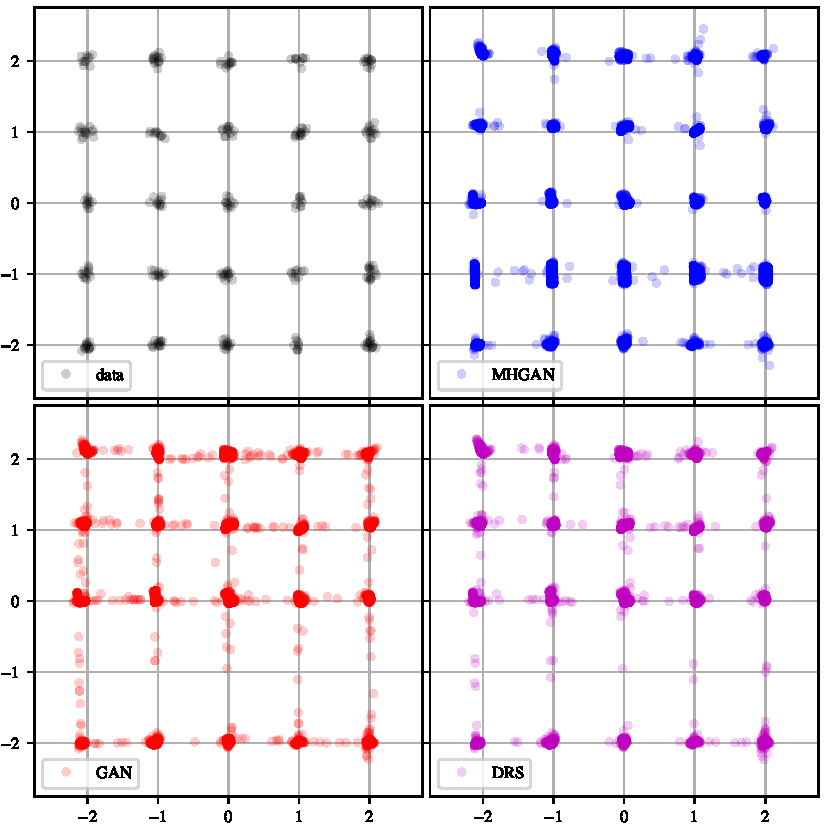
\includegraphics[width=.25\textwidth]{../figures/mog_example_150.pdf}
\end{figure}


\section*{\fontsize{67.1}{82} \selectfont \color{NavyBlue} Code \color{Black}}
\centering
\large {\url{https://github.com/TODO}}

\end{multicols}
\end{document}
